\chapter{Disseny}
\label{cha:dessign}

En aquest cap\'{i}tol veurem els patrons de dissenys emprats i les tecnologies implementades. Tamb\'{e} descriurem la interf\'{i}cie d'usuari m\'{e}s complexa i el fluxe de les operacions de sistema


\section{Esquema general l\`{o}gic arquitect\'{o}nic del sistema}
A continuaci\'{o} veiem un gr\`{a}fic amb els principals components del sistema i com es relacionen.

\begin{figure}[h]
  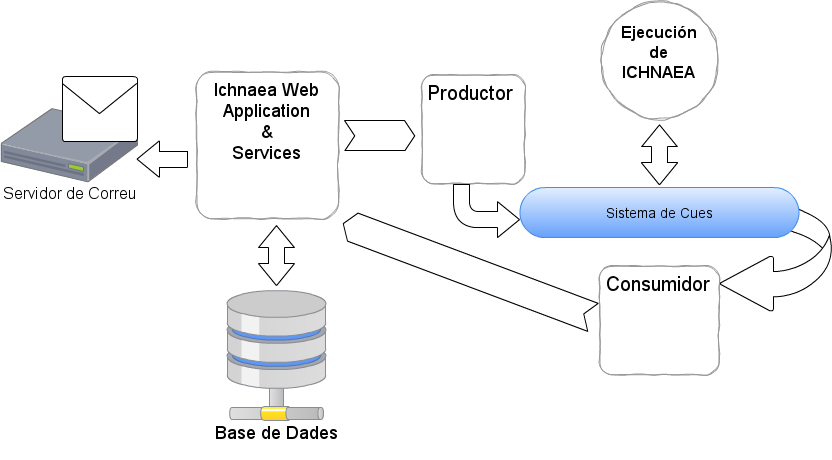
\includegraphics[scale=0.5]{img/design/ArchitectureSoftware.png}
  \caption{Arquitectura del sistema}
  \label{dessign:archsoftware}
\end{figure}
On:
\begin{itemize}
\item Ichnaea Web Application & Services: \'{e}s el \textit{core} de la aplicaci\'{o} i dels serveis HTTP.
\item Servidor de correu \'{e}s el servidor SMTP per enviar correus electr\`{o}nics als usuaris.
\item Productor-Cua-Consumidor \'{e}s el sistema de cues. Expliquem el paradigma al cap\'{i}tol \ref{sec:queue_system_overview} \ref{dessign:queue_system_overview}. La funci\'{o} \'{e}s gestionar els inicis, fluxes i finals d'execucions de Ichnaea.
\item La base de dades on es guardan els contiguts i models de dades i resultats.
\end{itemize}

\section{Patr\'{o} de disseny}
Per la implementaci\`{o} del sistema web s'han usat un disseny per capes(Presentaci\'{o}, domini i persistencia de dades) amb els seg\�{u}ents patrons de disseny:
  \begin{itemize}
  \item Model-Vista-Controlador amb controlador frontal
  \item Capa de Servei
  \item Injecci\'{o} de depend\`{e}ncies
  \item Repositori de model de dades
  \item Capa de mapejat de dades
  \item View template
  \item Interficies enriquides amb servei webs
  \end{itemize}

\subsection{Esquema del disseny}
La figura \ref{fig:dessignpatters} \'{e}s el diagrama general dels patrons que s'usaran per aquest projecte.
\begin{figure}[h]
  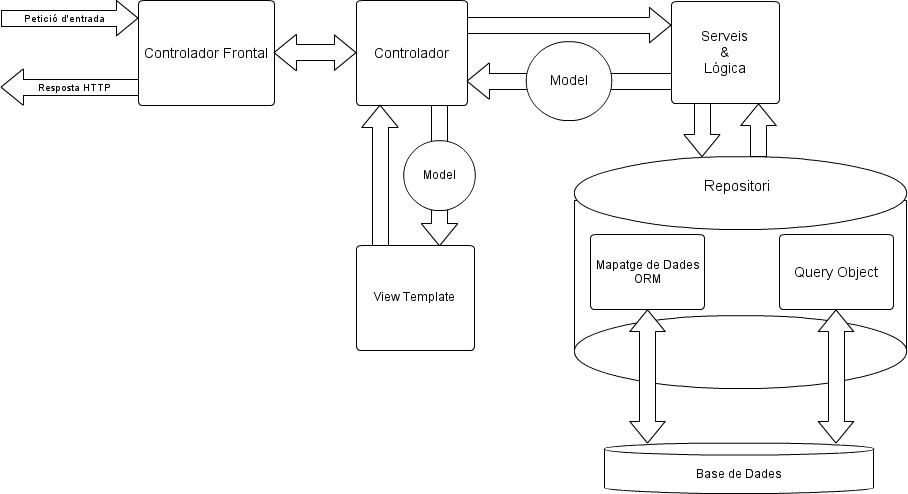
\includegraphics[scale=0.4]{img/design/IchnaeaPatterns.png}
  \caption{Patrons de disseny}
  \label{fig:dessignpatters}
\end{figure}

\subsection{Explicaci\'{o} del m\`{o}del}
Els components MVC,Model-Vista-Controlador, amb controlador frontal \'{e}s un disseny t\'{i}pic en les aplicacions web on:
\begin{itemize}
\item el model \'{e}s una representaci\'{o} de les dades en les que treballa la aplicaci\'{o}
\item la vista transforma el model a un format visible i llegible
\item el controlador frontal rep totes les peticions i les redirigeixs als controladors corresponents
\item el controlador se encarrega de processar les peticcions especifiques
\end{itemize}
L'arquitectura MVC separa la capa de presentaci\'{o} de la l\`{o}gica de domini. La capa de presentaci\'{o} accedeix a la capa de domini mitjan�ant serveis, injectant depend\'{e}ncies. \\
La injecci\'{o} de depend\'{e}ncies \'{e}s un patr\'{o} a on es suministren objectes a una clase en lloc de ser la clase qui crea els objectes\cite{dependency_injection}. Les avantatges de usuar DI(''dependency injection''):
\begin{itemize}
\item Codi m\'{e}s f\`{a}cil de mantenir, extendre o modificar
\item Desenvolupament guiat per proves (Test Driven Development o TDD en angl\'{e}s)
\item DI ens obliga a planejar una mica millor les nostres depend\`{e}ncies; decidim si una clase realment necesita d'un altre objecte per realitzar la seva funci�.
\end{itemize}
Els serveis, en aquest cas, contenen l\'{o}gica de Ichnaea. Accedeixen mitjan�ant les dades repositoris d'objectes. Els repositoris son mediadors entre el domini i les dades pesistents. Els repositoris retornen entitats de la l\'{ogica}. El mapatge de dades ORM(''Object Relational Mapping''), mapatge objecte-relacional, \'{e}s un patr\'{o} de disseny, encara que alguns enginyers els agrada dir que \'{e}s una tecnica de programaci\'{o} i a uns altres una tecnologia, que estableix una relaci\'{o} directe entre les entitats i la dades persistents.\cite{orm}

\section{Disseny d'interf\'{i}cies}
Les interf\'{i}cies s'ha dissenyat enriquides i 
\subsection{Interf\'{i}cie de configuraci\'{o} de matrius}
\subsection{Interficies de carrega de matrius per fitxers }
Per carregar les matrius s'ha emprat les noves funcionalitats HTML5 per llegir fitxers desde els propis clients web(navegadors). La selecci\'{o} de fitxers s'ha utilitzat la etiqueta <file> i els events BLAH BLAH. En una variable deshabilitada(en properes versions hauria de ser oculta) es carrega el contingut del fitxer.





